\documentclass[9pt,a4paper]{extarticle}
\usepackage{parskip}

\usepackage[utf8]{inputenc}
\usepackage[T1]{fontenc}
\usepackage[brazilian,provide=*]{babel}
\usepackage{amsmath, amssymb, amsthm}
\usepackage{geometry}
\usepackage{xcolor}
\usepackage{hyperref}
\usepackage{booktabs}
\usepackage{enumitem}
\usepackage[expansion=false]{microtype}
\usepackage{csquotes}
\usepackage{tikz}
\usetikzlibrary{positioning,arrows.meta}

\definecolor{important}{RGB}{255, 100, 100}
\definecolor{notice}{RGB}{0, 102, 204}
\definecolor{maccent}{RGB}{230, 120, 30}

\newcommand{\impt}[1]{\textcolor{important}{\textbf{#1}}}
\newcommand{\ntc}[1]{\textcolor{notice}{#1}}

\setlist{nosep}
\geometry{margin=2cm}

\newtheorem{theorem}{Teorema}[section]
\newtheorem{lemma}[theorem]{Lema}
\newtheorem{corollary}[theorem]{Corolário}
\theoremstyle{definition}
\newtheorem{definition}{Definição}[section]
\newtheorem{example}{Exemplo}[section]
\newtheorem{remark}{Observação}[section]
\newtheorem{exercise}{Exercício}[section]

\title{Material complementar: a redução \textsc{3-Cnf-Sat} \(\leq_p\) \textsc{Independent-Set}}
\author{PCC104 -- Projeto e Análise de Algoritmos}
\date{\today}

\begin{document}
\maketitle

\section{O que vamos provar, e por quê}

Nas notas principais provamos \textsc{3-Cnf-Sat} \(\leq_p\) \textsc{Clique} (Seção 7.1) e, logo no início (Seção 4), usamos como exemplo motivador a relação entre \textsc{Clique} e \textsc{Independent-Set} via grafo complementar. Este material fecha esse ciclo: vamos formalizar \textsc{Independent-Set} como problema de decisão e provar que ele também é NP-completo.

\begin{definition}[\textsc{Independent-Set}]
\textsc{Independent-Set}\((G,k)\): dado um grafo \(G=(V,E)\) e um inteiro \(k\), existe \(S \subseteq V\) com \(|S| = k\) tal que nenhum par de vértices de \(S\) é adjacente em \(G\)? Um conjunto \(S\) nessas condições é chamado \impt{conjunto independente}.
\end{definition}

\(\textsc{Independent-Set} \in NP\): o certificado é o próprio conjunto \(S\) candidato; o verificador checa os \(\binom{k}{2}\) pares -- polinomial.

\begin{remark}[Atenção com a direção]
Para provar que \textsc{Independent-Set} é NP-\emph{completo}, a direção da redução precisa ser \(\textsc{3-Cnf-Sat} \leq_p \textsc{Independent-Set}\) -- reduzimos um problema \emph{já sabidamente difícil} \emph{para} o problema que queremos classificar, exatamente como nas notas principais (Observação 4.3). Reduzir na direção contrária (\textsc{Independent-Set} \(\leq_p\) \textsc{3-Cnf-Sat}, isto é, \emph{codificar} uma instância de \textsc{Independent-Set} como fórmula SAT) é uma tarefa diferente, útil na prática para alimentar um SAT solver (Seção 8 das notas principais), mas não prova NP-completude de nada -- só mostra que \textsc{Independent-Set} não é mais difícil que \textsc{Sat}, o que já sabemos por outro caminho.
\end{remark}

\section{Duas rotas para a mesma prova}

\subsection{Rota A -- por transitividade (a rota curta)}

Não precisamos reinventar nada: já temos dois fatos provados.

\begin{enumerate}
\item (Seção 7.1 das notas principais) \(\textsc{3-Cnf-Sat} \leq_p \textsc{Clique}\), via a função \(g\) que constrói o grafo de triplos-de-cláusula.
\item (Seção 4 das notas principais) Para todo grafo \(G\) e inteiro \(k\): \(G\) tem clique de tamanho \(k\) \(\iff\) \(\bar G\) tem conjunto independente de tamanho \(k\). Isso já é, literalmente, uma redução \(\textsc{Clique} \leq_p \textsc{Independent-Set}\), via a função \(h(G,k) = (\bar G, k)\) (tomar o complementar).
\end{enumerate}

\begin{corollary}\label{cor:rota-a}
\(\textsc{3-Cnf-Sat} \leq_p \textsc{Independent-Set}\).
\end{corollary}
\begin{proof}
Pela transitividade das reduções (Lema 4.2 das notas principais), compor \(g\) seguida de \(h\) dá uma redução polinomial de \textsc{3-Cnf-Sat} para \textsc{Independent-Set}: a função composta \(f = h \circ g\) leva uma fórmula \(\phi\) primeiro ao grafo-de-triplos \(G_\phi\) (construção da Seção 7.1) e depois ao seu complementar \(\bar G_\phi\). Como cada etapa é polinomial e preserva a resposta (\enquote{sim} \(\to\) \enquote{sim}, \enquote{não} \(\to\) \enquote{não}), a composta também preserva.
\end{proof}

Isto já basta, junto com \(\textsc{Independent-Set} \in NP\), para concluir que \textsc{Independent-Set} é NP-completo (Corolário 5.2 das notas principais). \impt{A lição aqui}: uma vez que você tem reduções provadas, transitividade combina peças pequenas em resultados novos sem esforço extra -- não é preciso construir um gadget do zero toda vez.

\subsection{Rota B -- construção direta (a rota instrutiva)}

A função composta \(f = h \circ g\) da Rota A pode ser escrita como uma única construção direta, que vale a pena ver explicitamente: é \emph{exatamente} o grafo de triplos da Seção 7.1, mas com \impt{arestas e não-arestas trocadas}.

\paragraph{Construção.} Dada \(\phi = C_1 \wedge \dots \wedge C_k\) em FNC com 3 literais por cláusula, crie um triplo de vértices \(v_1^i,v_2^i,v_3^i\) por cláusula \(C_i\), exatamente como antes. Agora ligue \(v_p^i\) a \(v_q^j\) por uma aresta se, e somente se:
\begin{itemize}
\item[(a)] estão no \emph{mesmo} triplo (\(i=j\), \(p \neq q\)); \textbf{ou}
\item[(b)] os literais correspondentes são \emph{complementares} (um é \(x\), o outro \(\bar x\)).
\end{itemize}
Chame esse grafo de \(H_\phi\). A instância de \textsc{Independent-Set} é \((H_\phi, k)\).

\ntc{Compare com a Seção 7.1: lá, a aresta aparecia exatamente quando (a) e (b) \emph{falhavam} -- vértices de triplos diferentes com literais não complementares. Aqui é o oposto: \(H_\phi = \overline{G_\phi}\), o complementar do grafo da Clique. As duas construções carregam a mesma informação; só a regra de quando desenhar a aresta foi invertida.}

\begin{theorem}
\(\phi\) é satisfazível \(\iff\) \(H_\phi\) tem conjunto independente de tamanho \(k\).
\end{theorem}
\begin{proof}
(\(\Rightarrow\)) Se \(\phi\) é satisfazível, fixe uma atribuição satisfatória e escolha, em cada triplo, o vértice cujo literal é verdadeiro -- um vértice por triplo, \(k\) vértices ao todo. Esses \(k\) vértices não têm aresta (a) entre si (são de triplos distintos, por construção) nem aresta (b) (a atribuição não torna \(x\) e \(\bar x\) simultaneamente verdadeiros, então nunca escolhemos literais complementares). Logo formam um conjunto independente de tamanho \(k\).

(\(\Leftarrow\)) Se \(H_\phi\) tem conjunto independente \(S\) de tamanho \(k\): a ausência de arestas do tipo (a) força no máximo um vértice de \(S\) por triplo; como há exatamente \(k\) triplos e \(|S|=k\), \(S\) tem \emph{exatamente} um vértice por triplo. A ausência de arestas do tipo (b) garante que \(S\) nunca contém dois literais complementares. Atribua verdadeiro a cada literal escolhido por \(S\) (variáveis não escolhidas recebem valor arbitrário) -- essa atribuição é consistente e satisfaz toda cláusula, pois cada cláusula contribuiu com o literal do seu vértice em \(S\).
\end{proof}

A construção é polinomial: \(3k\) vértices, e testar cada um dos \(O(k^2)\) pares de vértices para as condições (a)/(b) custa tempo constante por par.

\section{Exemplo trabalhado}

Reaproveitando a mesma fórmula do Exemplo 7.1 das notas principais:
\[
\phi = (x_1 \vee x_2 \vee \bar x_3) \wedge (\bar x_1 \vee \bar x_2 \vee x_3), \qquad k = 2.
\]

Rotulando os vértices como antes -- \(a_1{=}x_1, a_2{=}x_2, a_3{=}\bar x_3\) (cláusula \(C_1\)) e \(b_1{=}\bar x_1, b_2{=}\bar x_2, b_3{=}x_3\) (cláusula \(C_2\)) --, o grafo \(H_\phi\) tem aresta em cada par \emph{do mesmo triplo} (\(a_1a_2, a_1a_3, a_2a_3, b_1b_2, b_1b_3, b_2b_3\)) e em cada par de \emph{literais complementares} (\(a_1b_1\), pois \(x_1,\bar x_1\); \(a_2b_2\), pois \(x_2,\bar x_2\); \(a_3b_3\), pois \(\bar x_3,x_3\)):

\begin{center}
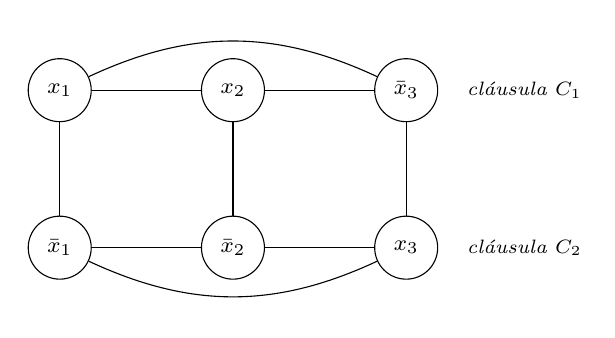
\begin{tikzpicture}[every node/.style={circle, draw, font=\footnotesize, inner sep=1.5pt, minimum size=8mm}]
\node (a1) at (0,2)   {\(x_1\)};
\node (a2) at (2.2,2) {\(x_2\)};
\node (a3) at (4.4,2) {\(\bar x_3\)};
\node (b1) at (0,0)   {\(\bar x_1\)};
\node (b2) at (2.2,0) {\(\bar x_2\)};
\node (b3) at (4.4,0) {\(x_3\)};
% arestas do mesmo triplo
\draw (a1) -- (a2);
\draw (a1) to[bend left=25] (a3);
\draw (a2) -- (a3);
\draw (b1) -- (b2);
\draw (b1) to[bend right=25] (b3);
\draw (b2) -- (b3);
% arestas de literais complementares
\draw (a1) -- (b1);
\draw (a2) -- (b2);
\draw (a3) -- (b3);
\node[draw=none, font=\scriptsize\itshape] at (5.9,2) {cláusula \(C_1\)};
\node[draw=none, font=\scriptsize\itshape] at (5.9,0) {cláusula \(C_2\)};
% destaque do conjunto independente (sem aresta entre eles)
\node[draw=none] at (0,1) {};
\end{tikzpicture}
\end{center}

Note que o par \(\{x_1, x_3\}\) = \(\{a_1, b_3\}\) \emph{não} tem aresta -- não são do mesmo triplo, e não são complementares -- então é um conjunto independente de tamanho \(k=2\). Corresponde exatamente à mesma atribuição satisfatória do Exemplo 7.1 (\(x_1=\mathrm{V}\), \(x_3=\mathrm{V}\)). \impt{Compare com o grafo \(G_\phi\) do Exemplo 7.1}: lá a clique era \(\{a_1,b_3\}\) porque \emph{havia} aresta entre eles; aqui o conjunto independente é o mesmo par de vértices porque \emph{não há} aresta -- exatamente a inversão que \(H_\phi = \overline{G_\phi}\) prevê.

\section{Exercício proposto}

\begin{exercise}
Considere \(\phi' = (x_1 \vee \bar x_2 \vee x_3) \wedge (\bar x_1 \vee x_2 \vee \bar x_3) \wedge (x_1 \vee x_2 \vee x_3)\), com \(k=3\).
\begin{enumerate}[label=(\alph*)]
\item Desenhe \(H_{\phi'}\) (9 vértices, 3 triplos), seguindo a regra de arestas desta seção.
\item Encontre uma atribuição que satisfaça \(\phi'\) e, a partir dela, exiba um conjunto independente de tamanho 3 em \(H_{\phi'}\).
\item Escolha um conjunto de 3 vértices, um por triplo, que \emph{não} seja independente (isto é, contenha um par de literais complementares) e explique por que a atribuição correspondente falha em satisfazer \(\phi'\).
\end{enumerate}
\end{exercise}

\end{document}